\paragraph{Git}
As stated by Komsiyski \cite{komsiyski2013binary}, Git works on basis of patch
files. As noted by Bryan \cite{bryan2018excuse}, large and often changing files
are not suitable for Git, since they can slow down pushes and pulls. According
to Perez et al. \cite{perez2016ten}, binary files in git are stored as a single
large entity. Therefore, even small changes lead to new copies in the
repository. This also makes it difficult to compare changes in files using diff
and may lead to frequent merge conflicts.

\paragraph{Git LFS}
Git also offers an extension for large files called Git LFS (Large File
Storage), which enables more efficient handling of large files
\cite{perez2016ten}. Content of the file is stored in cloud, with the repository
containing only pointers to the files, as noted in the documentation
\cite{gitlfs-structure} (Figure \ref{fig:gitlfs-architecture}). Since Git LFS is
a GitHub extension, its advantages are compatibility with Git
\cite{gitlfs-collaboration} and file agnosticism (compatibility with all file
formats) \cite{comparison}. Its disadvantages are inefficient storage management
- similar to Git, edited files are stored as new files. Therefore, it is not
suitable for large frequently-changing files, especially if they are compressed
(such as file formats frequently used in computer vision, e.g. jpg, png)
\cite{git-lfs}. In addition, data in Git LFS do not stay in place. It also does
not scale as well and its data retrieval is slow. As such, this approach is
suitable mostly for game developers and not for for ML and data science
purposes.

\begin{figure}[H]
    \centering
    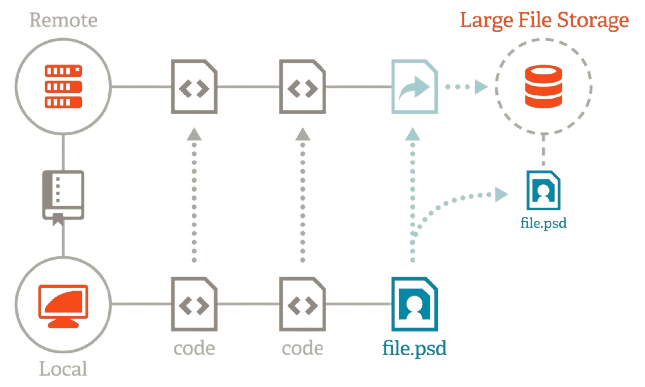
\includegraphics[width=0.8\textwidth]{fig/gitlfs-arch.png}
    \caption{Software architecture of Git LFS \cite{gitlfs-architecture}}
    \label{fig:gitlfs-architecture}
\end{figure}

\begin{comment}
Git offers a Large File Storage (LFS) module that
replaces such large files with pointers while the large binary file can be
stored remotely, which results in smaller and faster repositories. Git LFS is
also supported by GitHub, albeit with a space quota or for a fee, to retain your
usual GitHub workflow (https://help.github.com/categories/managing-large-files/)
(S1 File, Section 1).

GIT LFS (Large File Storage)

files above 50mb should be commited using Git LFS. 1 GiB of storage is free for
every account, together with 1GiB bandwidth. 5$ = 50 GiB storage, 50 GiB
bandwidth. text pointers are stored in git, the actual binary files are on cloud


https://www.atlassian.com/git/tutorials/git-lfs
https://docs.github.com/en/repositories/working-with-files/managing-large-files/about-storage-and-bandwidth-usage

When you commit and push a change to a file tracked with Git LFS, a new version
of the entire file is pushed and the total file size is counted against the
repository owner's storage limit. When you download a file tracked with Git LFS,
the total file size is counted against the repository owner's bandwidth limit.
Git LFS uploads do not count against the bandwidth limit.

For example:

If you push a 500 MB file to Git LFS, you'll use 500 MB of your allotted storage
and none of your bandwidth. If you make a 1 byte change and push the file again,
you'll use another 500 MB of storage and no bandwidth, bringing your total usage
for these two pushes to 1 GB of storage and zero bandwidth. If you download a
500 MB file that's tracked with LFS, you'll use 500 MB of the repository owner's
allotted bandwidth. If a collaborator pushes a change to the file and you pull
the new version to your local repository, you'll use another 500 MB of
bandwidth, bringing the total usage for these two downloads to 1 GB of
bandwidth. If GitHub Actions downloads a 500 MB file that is tracked with LFS,
it will use 500 MB of the repository owner's allotted bandwidth.
git works on basis of patch files, as Komsiyski states

\cite{komsiyski2013binary}, time for creating a patch and sending the patch to a
server has to be less than the time needed to send a new version of file to the
server.
\end{comment}